% ---------------------------------------------------------------------------
% Graph-clustering part of the 02807 report (Vishwaa).
% Include with % ---------------------------------------------------------------------------
% Graph-clustering part of the 02807 report (Vishwaa).
% Include with % ---------------------------------------------------------------------------
% Graph-clustering part of the 02807 report (Vishwaa).
% Include with % ---------------------------------------------------------------------------
% Graph-clustering part of the 02807 report (Vishwaa).
% Include with \input{graph_clustering} in main.tex.
% Needs in the preamble: \usepackage{amsmath,booktabs,graphicx}
% Figure file: recall_by_group.pdf (upload next to this file).
% Size: about 5,200 characters without spaces, of the 11,000 for the whole report.
% If this part sits under a bigger section, change \section -> \subsection
% and \subsection -> \subsubsection.
% ---------------------------------------------------------------------------

\section{Reader communities from book graphs}
\label{sec:graph}

We test whether books read by the same readers form communities that recommend
long-tail books better than purchase overlap (``readers also bought''), and
whether adding description similarity to the graph helps.
Graphs are built from the 1.74M reviews before 2014-01-01, after an iterative
$k$-core (users $\geq 5$, books $\geq 15$ reviews; 165k users, 52k books).
A review with rating $\geq 4$ counts as \emph{liked}.

\subsection{Book graphs}
From the sparse user$\times$book matrix $B$ we compute $C = B^\top W B$ block by
block, never as a dense all-pairs matrix. Using all reviews gives a
\emph{co-reader} graph (7.0M edges); using only liked reviews gives a
\emph{co-liked} graph (4.0M edges). An edge needs at least 2 shared readers.
Each user is weighted by $w_u = 1/\log(1+d_u)$, where $d_u$ is the number of
books they reviewed: without it, the 34 users with more than 500 books would
create 17.5\% of all book pairs. We implemented three edge weights: raw counts,
Jaccard $|U_i \cap U_j| / |U_i \cup U_j|$, which corrects for popularity, and
PPMI $\max\bigl(0, \log \tfrac{C_{ij}\,T}{r_i r_j}\bigr)$, which scores pairs that
co-occur more often than chance.

\subsection{Backbone: the disparity filter (outside the course)}
The graphs are too dense to cluster well, and a global weight threshold would
delete the long tail, whose edges are all light. The disparity filter
(Serrano, Bogu\~n\'a \& Vespignani, 2009) tests each edge against its own node.
Under the null model, a node with $k$ edges spreads its total weight $s$
uniformly at random, so an edge with share $p = w/s$ is at least this heavy with
probability
\begin{equation}
  \alpha_{ij} = (1 - p_{ij})^{\,k_i - 1}.
\end{equation}
An edge is kept if $\alpha_{ij}$ is below the threshold for either endpoint, so
every book keeps its own strongest links. A fixed threshold behaves very
differently per weighting: at $\alpha = 0.05$, raw counts keep 47\% of books but
PPMI only 3\%, because PPMI weights are nearly uniform around each node. We
therefore choose $\alpha$ per graph so that the backbone has as many edges as a
``top-10 neighbours'' baseline. The filter, the edge-budget matching and the
baseline are our own code.

\subsection{Clustering}
On the main backbone (co-liked, Jaccard, disparity filter; 309k edges, 95\% of
books connected) we ran Louvain for resolutions 0.5--20 with 5 seeds each.
Modularity peaks at 0.84 at resolution 1, and partitions from different seeds
agree with NMI 0.83. Our own spectral clustering (60 smallest eigenvectors of
$I - D^{-1/2} W D^{-1/2}$ on the 43.7k-book giant component, row-normalised,
then $k$-means) reaches modularity 0.71--0.75, so Louvain is used downstream.
Our modularity function matches networkx and igraph to 8 decimals.

\subsection{Recommender and evaluation}
For each reader, we recommend unread books from the communities of the books
they liked, ranked by their backbone links to those liked books. Ranking by
centrality inside a community, as first planned, gave everyone in a community
the same books and scored below ``most popular''. Baselines are \emph{most
popular} and \emph{item-kNN}, which sums raw co-reader counts with the user's
liked books, i.e.\ purchase overlap. A hybrid mixes the two as
$(1-\lambda)\,\text{kNN} + \lambda\,\text{community}$.
We measure recall@10 on books liked in January--July 2014, split by popularity
(head, mid and tail each hold a third of training interactions), and exclude
books from series the reader already read. Resolution, ranking and $\lambda$ were
chosen on 20\% of the test users; all results are on the other 59,392.

\subsection{Results}
The communities are coherent: NMI against Amazon genres is 0.29 versus 0.06
for random partitions of equal sizes. 12 of the 39 large labelled communities
mix genres in ways that make sense to readers, e.g.\ post-apocalyptic thrillers
with prepper manuals, or clean romance with Christian fiction.

\begin{table}[ht]
  \centering
  \small
  \begin{tabular}{lrrrrr}
    \toprule
    Method & Recall@10 & Head & Mid & Tail & Coverage \\
    \midrule
    Most popular                  & 0.008          & 0.021          & 0              & 0              & 0.04\% \\
    Item-kNN (purchase overlap)   & 0.035          & \textbf{0.072} & 0.022          & 0.009          & 47\%   \\
    Community                     & 0.039          & 0.044          & 0.038          & 0.027          & 82\%   \\
    Hybrid ($\lambda = 0.5$)      & 0.041          & 0.064          & 0.034          & 0.020          & 73\%   \\
    Backbone-kNN (no communities) & 0.039          & 0.044          & 0.038          & 0.027          & 84\%   \\
    \midrule
    Community, combined graph     & 0.039          & 0.043          & \textbf{0.038} & \textbf{0.029} & 84\%   \\
    Hybrid, combined ($\lambda = 0.7$) & \textbf{0.041} & 0.056     & 0.037          & 0.025          & 80\%   \\
    \bottomrule
  \end{tabular}
  \caption{Recommendation quality on 59,392 held-out readers, books from series
  the reader already read removed. Coverage is the share of the catalogue that is
  recommended to at least one reader. The last two rows add description
  similarity to the graph (Section~\ref{sec:content}).}
  \label{tab:recs}
\end{table}

\begin{figure}[ht]
  \centering
  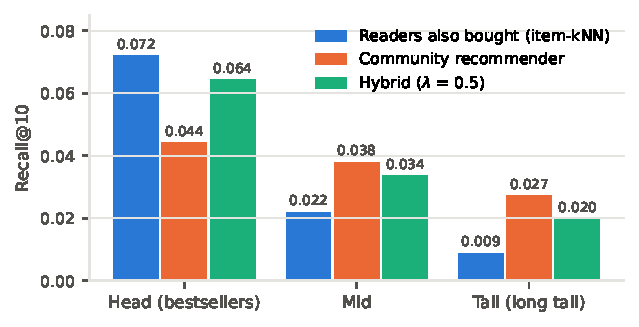
\includegraphics[width=0.8\linewidth]{recall_by_group.pdf}
  \caption{Recall@10 by book popularity group. Purchase overlap wins on
  bestsellers; the graph recommenders win on the middle and the long tail.}
  \label{fig:recall}
\end{figure}

Against item-kNN, the community recommender raises recall by 9\% (95\%
bootstrap CI 6--13\%) and finds long-tail books 3.1 times as often
(Table~\ref{tab:recs}, Figure~\ref{fig:recall}). 81\% of item-kNN's
recommendations are bestsellers, against 38\% for the community recommender.
The hybrid gains 16\% overall while losing only 11\% on the head.

\subsection{Adding description similarity}
\label{sec:content}
The similarity part compares books by their descriptions (SBERT
all-MiniLM-L6-v2 embeddings, cosine). We turned it into a graph in which each of
the 33.5k training books with a description keeps its 10 most similar books;
only 5.6\% of these edges are also backbone edges. We cluster the union
$0.75\,\tilde{D} + 0.25\,\tilde{T}$ of the co-liked backbone and this content
graph, each divided by its mean edge weight, with the share chosen on
validation users. Alone, the content graph is a weak recommender (recall@10
0.013): a similar description says what a book is about, not who reads it.
Combined, it raises the community recommender's tail recall from 0.027 to 0.029
(+6\%, CI 4--8\%) at unchanged overall recall.

\subsection{Discussion}
The graph method meets its goal on the long tail. On the reader graph alone the
community step adds no accuracy: recommending from the same backbone without
communities scores the same (difference $+0.0001$, CI $-0.0003$ to $+0.0004$),
because 91\% of the backbone's edge weight already lies inside communities. On
the combined graph this share falls to 68\%, and the communities beat the same
graph without them by 1.3\% (CI 0.3--2.4\%): restricting to a community filters
out description links between books with different readers. Clustering also
gives interpretable reader communities and a compact summary of the graph.
Limitations: the data is from 2014, reviews only approximate purchases, only
18\% of books have a genre, and the series check is approximate.
 in main.tex.
% Needs in the preamble: \usepackage{amsmath,booktabs,graphicx}
% Figure file: recall_by_group.pdf (upload next to this file).
% Size: about 5,200 characters without spaces, of the 11,000 for the whole report.
% If this part sits under a bigger section, change \section -> \subsection
% and \subsection -> \subsubsection.
% ---------------------------------------------------------------------------

\section{Reader communities from book graphs}
\label{sec:graph}

We test whether books read by the same readers form communities that recommend
long-tail books better than purchase overlap (``readers also bought''), and
whether adding description similarity to the graph helps.
Graphs are built from the 1.74M reviews before 2014-01-01, after an iterative
$k$-core (users $\geq 5$, books $\geq 15$ reviews; 165k users, 52k books).
A review with rating $\geq 4$ counts as \emph{liked}.

\subsection{Book graphs}
From the sparse user$\times$book matrix $B$ we compute $C = B^\top W B$ block by
block, never as a dense all-pairs matrix. Using all reviews gives a
\emph{co-reader} graph (7.0M edges); using only liked reviews gives a
\emph{co-liked} graph (4.0M edges). An edge needs at least 2 shared readers.
Each user is weighted by $w_u = 1/\log(1+d_u)$, where $d_u$ is the number of
books they reviewed: without it, the 34 users with more than 500 books would
create 17.5\% of all book pairs. We implemented three edge weights: raw counts,
Jaccard $|U_i \cap U_j| / |U_i \cup U_j|$, which corrects for popularity, and
PPMI $\max\bigl(0, \log \tfrac{C_{ij}\,T}{r_i r_j}\bigr)$, which scores pairs that
co-occur more often than chance.

\subsection{Backbone: the disparity filter (outside the course)}
The graphs are too dense to cluster well, and a global weight threshold would
delete the long tail, whose edges are all light. The disparity filter
(Serrano, Bogu\~n\'a \& Vespignani, 2009) tests each edge against its own node.
Under the null model, a node with $k$ edges spreads its total weight $s$
uniformly at random, so an edge with share $p = w/s$ is at least this heavy with
probability
\begin{equation}
  \alpha_{ij} = (1 - p_{ij})^{\,k_i - 1}.
\end{equation}
An edge is kept if $\alpha_{ij}$ is below the threshold for either endpoint, so
every book keeps its own strongest links. A fixed threshold behaves very
differently per weighting: at $\alpha = 0.05$, raw counts keep 47\% of books but
PPMI only 3\%, because PPMI weights are nearly uniform around each node. We
therefore choose $\alpha$ per graph so that the backbone has as many edges as a
``top-10 neighbours'' baseline. The filter, the edge-budget matching and the
baseline are our own code.

\subsection{Clustering}
On the main backbone (co-liked, Jaccard, disparity filter; 309k edges, 95\% of
books connected) we ran Louvain for resolutions 0.5--20 with 5 seeds each.
Modularity peaks at 0.84 at resolution 1, and partitions from different seeds
agree with NMI 0.83. Our own spectral clustering (60 smallest eigenvectors of
$I - D^{-1/2} W D^{-1/2}$ on the 43.7k-book giant component, row-normalised,
then $k$-means) reaches modularity 0.71--0.75, so Louvain is used downstream.
Our modularity function matches networkx and igraph to 8 decimals.

\subsection{Recommender and evaluation}
For each reader, we recommend unread books from the communities of the books
they liked, ranked by their backbone links to those liked books. Ranking by
centrality inside a community, as first planned, gave everyone in a community
the same books and scored below ``most popular''. Baselines are \emph{most
popular} and \emph{item-kNN}, which sums raw co-reader counts with the user's
liked books, i.e.\ purchase overlap. A hybrid mixes the two as
$(1-\lambda)\,\text{kNN} + \lambda\,\text{community}$.
We measure recall@10 on books liked in January--July 2014, split by popularity
(head, mid and tail each hold a third of training interactions), and exclude
books from series the reader already read. Resolution, ranking and $\lambda$ were
chosen on 20\% of the test users; all results are on the other 59,392.

\subsection{Results}
The communities are coherent: NMI against Amazon genres is 0.29 versus 0.06
for random partitions of equal sizes. 12 of the 39 large labelled communities
mix genres in ways that make sense to readers, e.g.\ post-apocalyptic thrillers
with prepper manuals, or clean romance with Christian fiction.

\begin{table}[ht]
  \centering
  \small
  \begin{tabular}{lrrrrr}
    \toprule
    Method & Recall@10 & Head & Mid & Tail & Coverage \\
    \midrule
    Most popular                  & 0.008          & 0.021          & 0              & 0              & 0.04\% \\
    Item-kNN (purchase overlap)   & 0.035          & \textbf{0.072} & 0.022          & 0.009          & 47\%   \\
    Community                     & 0.039          & 0.044          & 0.038          & 0.027          & 82\%   \\
    Hybrid ($\lambda = 0.5$)      & 0.041          & 0.064          & 0.034          & 0.020          & 73\%   \\
    Backbone-kNN (no communities) & 0.039          & 0.044          & 0.038          & 0.027          & 84\%   \\
    \midrule
    Community, combined graph     & 0.039          & 0.043          & \textbf{0.038} & \textbf{0.029} & 84\%   \\
    Hybrid, combined ($\lambda = 0.7$) & \textbf{0.041} & 0.056     & 0.037          & 0.025          & 80\%   \\
    \bottomrule
  \end{tabular}
  \caption{Recommendation quality on 59,392 held-out readers, books from series
  the reader already read removed. Coverage is the share of the catalogue that is
  recommended to at least one reader. The last two rows add description
  similarity to the graph (Section~\ref{sec:content}).}
  \label{tab:recs}
\end{table}

\begin{figure}[ht]
  \centering
  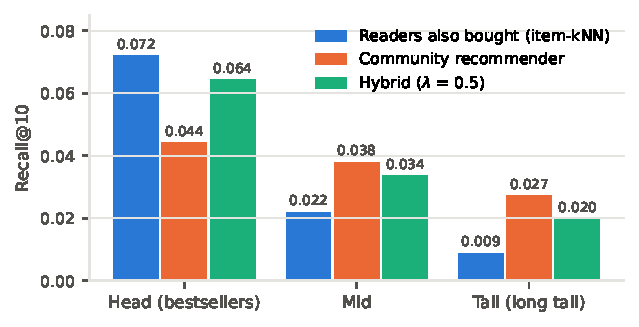
\includegraphics[width=0.8\linewidth]{recall_by_group.pdf}
  \caption{Recall@10 by book popularity group. Purchase overlap wins on
  bestsellers; the graph recommenders win on the middle and the long tail.}
  \label{fig:recall}
\end{figure}

Against item-kNN, the community recommender raises recall by 9\% (95\%
bootstrap CI 6--13\%) and finds long-tail books 3.1 times as often
(Table~\ref{tab:recs}, Figure~\ref{fig:recall}). 81\% of item-kNN's
recommendations are bestsellers, against 38\% for the community recommender.
The hybrid gains 16\% overall while losing only 11\% on the head.

\subsection{Adding description similarity}
\label{sec:content}
The similarity part compares books by their descriptions (SBERT
all-MiniLM-L6-v2 embeddings, cosine). We turned it into a graph in which each of
the 33.5k training books with a description keeps its 10 most similar books;
only 5.6\% of these edges are also backbone edges. We cluster the union
$0.75\,\tilde{D} + 0.25\,\tilde{T}$ of the co-liked backbone and this content
graph, each divided by its mean edge weight, with the share chosen on
validation users. Alone, the content graph is a weak recommender (recall@10
0.013): a similar description says what a book is about, not who reads it.
Combined, it raises the community recommender's tail recall from 0.027 to 0.029
(+6\%, CI 4--8\%) at unchanged overall recall.

\subsection{Discussion}
The graph method meets its goal on the long tail. On the reader graph alone the
community step adds no accuracy: recommending from the same backbone without
communities scores the same (difference $+0.0001$, CI $-0.0003$ to $+0.0004$),
because 91\% of the backbone's edge weight already lies inside communities. On
the combined graph this share falls to 68\%, and the communities beat the same
graph without them by 1.3\% (CI 0.3--2.4\%): restricting to a community filters
out description links between books with different readers. Clustering also
gives interpretable reader communities and a compact summary of the graph.
Limitations: the data is from 2014, reviews only approximate purchases, only
18\% of books have a genre, and the series check is approximate.
 in main.tex.
% Needs in the preamble: \usepackage{amsmath,booktabs,graphicx}
% Figure file: recall_by_group.pdf (upload next to this file).
% Size: about 5,200 characters without spaces, of the 11,000 for the whole report.
% If this part sits under a bigger section, change \section -> \subsection
% and \subsection -> \subsubsection.
% ---------------------------------------------------------------------------

\section{Reader communities from book graphs}
\label{sec:graph}

We test whether books read by the same readers form communities that recommend
long-tail books better than purchase overlap (``readers also bought''), and
whether adding description similarity to the graph helps.
Graphs are built from the 1.74M reviews before 2014-01-01, after an iterative
$k$-core (users $\geq 5$, books $\geq 15$ reviews; 165k users, 52k books).
A review with rating $\geq 4$ counts as \emph{liked}.

\subsection{Book graphs}
From the sparse user$\times$book matrix $B$ we compute $C = B^\top W B$ block by
block, never as a dense all-pairs matrix. Using all reviews gives a
\emph{co-reader} graph (7.0M edges); using only liked reviews gives a
\emph{co-liked} graph (4.0M edges). An edge needs at least 2 shared readers.
Each user is weighted by $w_u = 1/\log(1+d_u)$, where $d_u$ is the number of
books they reviewed: without it, the 34 users with more than 500 books would
create 17.5\% of all book pairs. We implemented three edge weights: raw counts,
Jaccard $|U_i \cap U_j| / |U_i \cup U_j|$, which corrects for popularity, and
PPMI $\max\bigl(0, \log \tfrac{C_{ij}\,T}{r_i r_j}\bigr)$, which scores pairs that
co-occur more often than chance.

\subsection{Backbone: the disparity filter (outside the course)}
The graphs are too dense to cluster well, and a global weight threshold would
delete the long tail, whose edges are all light. The disparity filter
(Serrano, Bogu\~n\'a \& Vespignani, 2009) tests each edge against its own node.
Under the null model, a node with $k$ edges spreads its total weight $s$
uniformly at random, so an edge with share $p = w/s$ is at least this heavy with
probability
\begin{equation}
  \alpha_{ij} = (1 - p_{ij})^{\,k_i - 1}.
\end{equation}
An edge is kept if $\alpha_{ij}$ is below the threshold for either endpoint, so
every book keeps its own strongest links. A fixed threshold behaves very
differently per weighting: at $\alpha = 0.05$, raw counts keep 47\% of books but
PPMI only 3\%, because PPMI weights are nearly uniform around each node. We
therefore choose $\alpha$ per graph so that the backbone has as many edges as a
``top-10 neighbours'' baseline. The filter, the edge-budget matching and the
baseline are our own code.

\subsection{Clustering}
On the main backbone (co-liked, Jaccard, disparity filter; 309k edges, 95\% of
books connected) we ran Louvain for resolutions 0.5--20 with 5 seeds each.
Modularity peaks at 0.84 at resolution 1, and partitions from different seeds
agree with NMI 0.83. Our own spectral clustering (60 smallest eigenvectors of
$I - D^{-1/2} W D^{-1/2}$ on the 43.7k-book giant component, row-normalised,
then $k$-means) reaches modularity 0.71--0.75, so Louvain is used downstream.
Our modularity function matches networkx and igraph to 8 decimals.

\subsection{Recommender and evaluation}
For each reader, we recommend unread books from the communities of the books
they liked, ranked by their backbone links to those liked books. Ranking by
centrality inside a community, as first planned, gave everyone in a community
the same books and scored below ``most popular''. Baselines are \emph{most
popular} and \emph{item-kNN}, which sums raw co-reader counts with the user's
liked books, i.e.\ purchase overlap. A hybrid mixes the two as
$(1-\lambda)\,\text{kNN} + \lambda\,\text{community}$.
We measure recall@10 on books liked in January--July 2014, split by popularity
(head, mid and tail each hold a third of training interactions), and exclude
books from series the reader already read. Resolution, ranking and $\lambda$ were
chosen on 20\% of the test users; all results are on the other 59,392.

\subsection{Results}
The communities are coherent: NMI against Amazon genres is 0.29 versus 0.06
for random partitions of equal sizes. 12 of the 39 large labelled communities
mix genres in ways that make sense to readers, e.g.\ post-apocalyptic thrillers
with prepper manuals, or clean romance with Christian fiction.

\begin{table}[ht]
  \centering
  \small
  \begin{tabular}{lrrrrr}
    \toprule
    Method & Recall@10 & Head & Mid & Tail & Coverage \\
    \midrule
    Most popular                  & 0.008          & 0.021          & 0              & 0              & 0.04\% \\
    Item-kNN (purchase overlap)   & 0.035          & \textbf{0.072} & 0.022          & 0.009          & 47\%   \\
    Community                     & 0.039          & 0.044          & 0.038          & 0.027          & 82\%   \\
    Hybrid ($\lambda = 0.5$)      & 0.041          & 0.064          & 0.034          & 0.020          & 73\%   \\
    Backbone-kNN (no communities) & 0.039          & 0.044          & 0.038          & 0.027          & 84\%   \\
    \midrule
    Community, combined graph     & 0.039          & 0.043          & \textbf{0.038} & \textbf{0.029} & 84\%   \\
    Hybrid, combined ($\lambda = 0.7$) & \textbf{0.041} & 0.056     & 0.037          & 0.025          & 80\%   \\
    \bottomrule
  \end{tabular}
  \caption{Recommendation quality on 59,392 held-out readers, books from series
  the reader already read removed. Coverage is the share of the catalogue that is
  recommended to at least one reader. The last two rows add description
  similarity to the graph (Section~\ref{sec:content}).}
  \label{tab:recs}
\end{table}

\begin{figure}[ht]
  \centering
  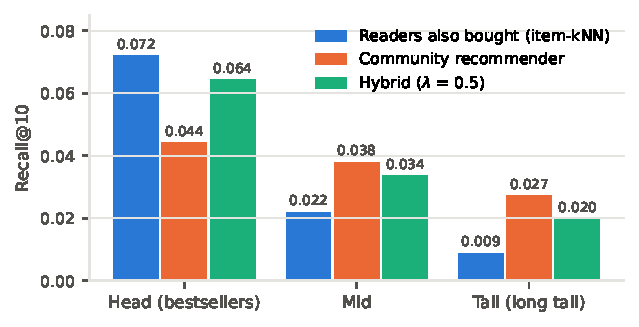
\includegraphics[width=0.8\linewidth]{recall_by_group.pdf}
  \caption{Recall@10 by book popularity group. Purchase overlap wins on
  bestsellers; the graph recommenders win on the middle and the long tail.}
  \label{fig:recall}
\end{figure}

Against item-kNN, the community recommender raises recall by 9\% (95\%
bootstrap CI 6--13\%) and finds long-tail books 3.1 times as often
(Table~\ref{tab:recs}, Figure~\ref{fig:recall}). 81\% of item-kNN's
recommendations are bestsellers, against 38\% for the community recommender.
The hybrid gains 16\% overall while losing only 11\% on the head.

\subsection{Adding description similarity}
\label{sec:content}
The similarity part compares books by their descriptions (SBERT
all-MiniLM-L6-v2 embeddings, cosine). We turned it into a graph in which each of
the 33.5k training books with a description keeps its 10 most similar books;
only 5.6\% of these edges are also backbone edges. We cluster the union
$0.75\,\tilde{D} + 0.25\,\tilde{T}$ of the co-liked backbone and this content
graph, each divided by its mean edge weight, with the share chosen on
validation users. Alone, the content graph is a weak recommender (recall@10
0.013): a similar description says what a book is about, not who reads it.
Combined, it raises the community recommender's tail recall from 0.027 to 0.029
(+6\%, CI 4--8\%) at unchanged overall recall.

\subsection{Discussion}
The graph method meets its goal on the long tail. On the reader graph alone the
community step adds no accuracy: recommending from the same backbone without
communities scores the same (difference $+0.0001$, CI $-0.0003$ to $+0.0004$),
because 91\% of the backbone's edge weight already lies inside communities. On
the combined graph this share falls to 68\%, and the communities beat the same
graph without them by 1.3\% (CI 0.3--2.4\%): restricting to a community filters
out description links between books with different readers. Clustering also
gives interpretable reader communities and a compact summary of the graph.
Limitations: the data is from 2014, reviews only approximate purchases, only
18\% of books have a genre, and the series check is approximate.
 in main.tex.
% Needs in the preamble: \usepackage{amsmath,booktabs,graphicx}
% Figure file: recall_by_group.pdf (upload next to this file).
% Size: about 5,200 characters without spaces, of the 11,000 for the whole report.
% If this part sits under a bigger section, change \section -> \subsection
% and \subsection -> \subsubsection.
% ---------------------------------------------------------------------------

\section{Reader communities from book graphs}
\label{sec:graph}

We test whether books read by the same readers form communities that recommend
long-tail books better than purchase overlap (``readers also bought''), and
whether adding description similarity to the graph helps.
Graphs are built from the 1.74M reviews before 2014-01-01, after an iterative
$k$-core (users $\geq 5$, books $\geq 15$ reviews; 165k users, 52k books).
A review with rating $\geq 4$ counts as \emph{liked}.

\subsection{Book graphs}
From the sparse user$\times$book matrix $B$ we compute $C = B^\top W B$ block by
block, never as a dense all-pairs matrix. Using all reviews gives a
\emph{co-reader} graph (7.0M edges); using only liked reviews gives a
\emph{co-liked} graph (4.0M edges). An edge needs at least 2 shared readers.
Each user is weighted by $w_u = 1/\log(1+d_u)$, where $d_u$ is the number of
books they reviewed: without it, the 34 users with more than 500 books would
create 17.5\% of all book pairs. We implemented three edge weights: raw counts,
Jaccard $|U_i \cap U_j| / |U_i \cup U_j|$, which corrects for popularity, and
PPMI $\max\bigl(0, \log \tfrac{C_{ij}\,T}{r_i r_j}\bigr)$, which scores pairs that
co-occur more often than chance.

\subsection{Backbone: the disparity filter (outside the course)}
The graphs are too dense to cluster well, and a global weight threshold would
delete the long tail, whose edges are all light. The disparity filter
(Serrano, Bogu\~n\'a \& Vespignani, 2009) tests each edge against its own node.
Under the null model, a node with $k$ edges spreads its total weight $s$
uniformly at random, so an edge with share $p = w/s$ is at least this heavy with
probability
\begin{equation}
  \alpha_{ij} = (1 - p_{ij})^{\,k_i - 1}.
\end{equation}
An edge is kept if $\alpha_{ij}$ is below the threshold for either endpoint, so
every book keeps its own strongest links. A fixed threshold behaves very
differently per weighting: at $\alpha = 0.05$, raw counts keep 47\% of books but
PPMI only 3\%, because PPMI weights are nearly uniform around each node. We
therefore choose $\alpha$ per graph so that the backbone has as many edges as a
``top-10 neighbours'' baseline. The filter, the edge-budget matching and the
baseline are our own code.

\subsection{Clustering}
On the main backbone (co-liked, Jaccard, disparity filter; 309k edges, 95\% of
books connected) we ran Louvain for resolutions 0.5--20 with 5 seeds each.
Modularity peaks at 0.84 at resolution 1, and partitions from different seeds
agree with NMI 0.83. Our own spectral clustering (60 smallest eigenvectors of
$I - D^{-1/2} W D^{-1/2}$ on the 43.7k-book giant component, row-normalised,
then $k$-means) reaches modularity 0.71--0.75, so Louvain is used downstream.
Our modularity function matches networkx and igraph to 8 decimals.

\subsection{Recommender and evaluation}
For each reader, we recommend unread books from the communities of the books
they liked, ranked by their backbone links to those liked books. Ranking by
centrality inside a community, as first planned, gave everyone in a community
the same books and scored below ``most popular''. Baselines are \emph{most
popular} and \emph{item-kNN}, which sums raw co-reader counts with the user's
liked books, i.e.\ purchase overlap. A hybrid mixes the two as
$(1-\lambda)\,\text{kNN} + \lambda\,\text{community}$.
We measure recall@10 on books liked in January--July 2014, split by popularity
(head, mid and tail each hold a third of training interactions), and exclude
books from series the reader already read. Resolution, ranking and $\lambda$ were
chosen on 20\% of the test users; all results are on the other 59,392.

\subsection{Results}
The communities are coherent: NMI against Amazon genres is 0.29 versus 0.06
for random partitions of equal sizes. 12 of the 39 large labelled communities
mix genres in ways that make sense to readers, e.g.\ post-apocalyptic thrillers
with prepper manuals, or clean romance with Christian fiction.

\begin{table}[ht]
  \centering
  \small
  \begin{tabular}{lrrrrr}
    \toprule
    Method & Recall@10 & Head & Mid & Tail & Coverage \\
    \midrule
    Most popular                  & 0.008          & 0.021          & 0              & 0              & 0.04\% \\
    Item-kNN (purchase overlap)   & 0.035          & \textbf{0.072} & 0.022          & 0.009          & 47\%   \\
    Community                     & 0.039          & 0.044          & 0.038          & 0.027          & 82\%   \\
    Hybrid ($\lambda = 0.5$)      & 0.041          & 0.064          & 0.034          & 0.020          & 73\%   \\
    Backbone-kNN (no communities) & 0.039          & 0.044          & 0.038          & 0.027          & 84\%   \\
    \midrule
    Community, combined graph     & 0.039          & 0.043          & \textbf{0.038} & \textbf{0.029} & 84\%   \\
    Hybrid, combined ($\lambda = 0.7$) & \textbf{0.041} & 0.056     & 0.037          & 0.025          & 80\%   \\
    \bottomrule
  \end{tabular}
  \caption{Recommendation quality on 59,392 held-out readers, books from series
  the reader already read removed. Coverage is the share of the catalogue that is
  recommended to at least one reader. The last two rows add description
  similarity to the graph (Section~\ref{sec:content}).}
  \label{tab:recs}
\end{table}

\begin{figure}[ht]
  \centering
  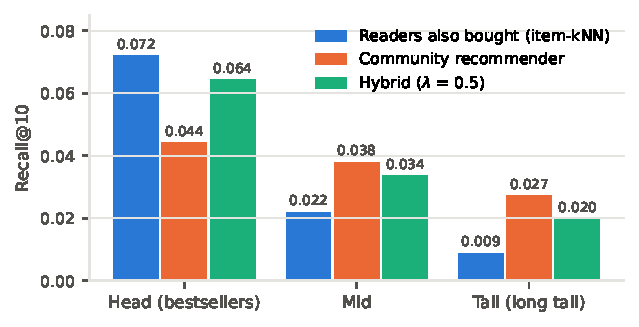
\includegraphics[width=0.8\linewidth]{recall_by_group.pdf}
  \caption{Recall@10 by book popularity group. Purchase overlap wins on
  bestsellers; the graph recommenders win on the middle and the long tail.}
  \label{fig:recall}
\end{figure}

Against item-kNN, the community recommender raises recall by 9\% (95\%
bootstrap CI 6--13\%) and finds long-tail books 3.1 times as often
(Table~\ref{tab:recs}, Figure~\ref{fig:recall}). 81\% of item-kNN's
recommendations are bestsellers, against 38\% for the community recommender.
The hybrid gains 16\% overall while losing only 11\% on the head.

\subsection{Adding description similarity}
\label{sec:content}
The similarity part compares books by their descriptions (SBERT
all-MiniLM-L6-v2 embeddings, cosine). We turned it into a graph in which each of
the 33.5k training books with a description keeps its 10 most similar books;
only 5.6\% of these edges are also backbone edges. We cluster the union
$0.75\,\tilde{D} + 0.25\,\tilde{T}$ of the co-liked backbone and this content
graph, each divided by its mean edge weight, with the share chosen on
validation users. Alone, the content graph is a weak recommender (recall@10
0.013): a similar description says what a book is about, not who reads it.
Combined, it raises the community recommender's tail recall from 0.027 to 0.029
(+6\%, CI 4--8\%) at unchanged overall recall.

\subsection{Discussion}
The graph method meets its goal on the long tail. On the reader graph alone the
community step adds no accuracy: recommending from the same backbone without
communities scores the same (difference $+0.0001$, CI $-0.0003$ to $+0.0004$),
because 91\% of the backbone's edge weight already lies inside communities. On
the combined graph this share falls to 68\%, and the communities beat the same
graph without them by 1.3\% (CI 0.3--2.4\%): restricting to a community filters
out description links between books with different readers. Clustering also
gives interpretable reader communities and a compact summary of the graph.
Limitations: the data is from 2014, reviews only approximate purchases, only
18\% of books have a genre, and the series check is approximate.
